Which characteristics of the use of smartphones
in web surveys are researched on and what are research gaps in the field?

To get an overview of the research on smartphone use in web surveys, we are going to analyse the topics of the selected articles in this review and the complementary meta data extracted in the search process. These insights will allow us to better understand the research field and to identify research gaps. 

In the final search results subset we identified 86 relevant papers from which 84 articles where published in a peer reviewed journal and 2 where published in peer reviewed conference proceedings. When looking at figure \ref{fig: publications_per_year_per_categories} we can see that before 2013 the was only limited research on this topic and an increasing trend of publications from 2013 until 2019. From 2020 on the trend seemed to be stopped and the publication count stagnates on a lower level. This trend reflects the increasing importance of participants using smartphone to access web surveys since and the general trend of increase usage of mobile devices to access online content (\cite{weigold_computerized_2021}). One weakness of this research area is the strong time bound of results, as the behaviour of smartphone user is continuously changing as user demographics and other influencing factors are changing \cite{broel_desktop_2018}. As this trend continues in the next year, we expect further and growing interest in the role of smartphones and other smart devices in surveys and data collection.  

In the extraction of the information from selected articles, we assigned each article one or more topics, that are presented in figure \ref{fig: publications_per_year_per_categories}. We identified seven categories of article contents including one meta category (reviews). 

Research articles with the subject data quality investigate quality indicators for smartphone web survey participants. Reading the articles we identified the pattern, that mobile web survey data quality is mainly measured in comparison with data quality on PC web surveys \cite{de_bruijne_comparing_2013, ha_data_2020}. The topics mobile participants mainly features research on the characteristics of participants of web surveys, that decide to take them on their smartphone. While the topic online participants investigate which participants of online surveys would be willing or want to participate with their mobile phone. The mobile design category comprises articles that examine how different design elements like grids, button and other are working on mobile devices and how they have to be adjusted for the use on smartphones. Articles considering input alternatives explore potential extension of web surveys with smartphone characteristic input possibilities like voice recording or movement data. Another aspect of survey research design invitation mode, includes paper that test the influence of different invitation modes on smartphone web survey participants. The last (meta) category reviews, are articles that review all or part of the prior topics from a scientific perspective. 

\begin{figure}
    \centering
    \includegraphics[width=\textwidth]{reports/figures/publications_per_year_per_categories.png}
     \caption{Graphic of the number of published articles per year per category of approach in the selected literature from 2008 to 2021}
    \label{fig: publications_per_year_per_categories}
\end{figure}

We are going to analyse the various topics in more detail in the next two section. For this we decide to cluster the topics into two categories Survey Design and Survey Quality. Survey Design comprises all decision in the design of a survey as mobile design, input alternatives and invitation mode, while Survey Quality comprises all the quality dimension: data quality, mobile and online participants. We could not identify missing research topics on this level on granularity. However, we will discuss research gaps in the identified categories in the next two sections. 

In the rest of this section we analyse the meta data of the results of the systematic search. This will help us to identify research gaps and to critically evaluate existing research.

An interesting observation, that is important for our evaluation of the dimensions of mobile web surveys, is the time difference between publication and data collection. As 74 articles in the review collected survey data, the time of survey taking is important for the evaluation of the results. When analyzing the year of survey execution we could identify an average gap between publication year and survey execution year of three years. This implies an important time lag of the data and the insights we gain in this review. As the latest survey was done in 2019 and 90\% of the survey were done in or before 2017. That is a significant difference that needs to be kept in mind when interpreting the results.  

As only two publication were in conference proceedings and the large majority of articles were published in journals we will limit us to an analysis of the published journals. As one can observe in table \ref{tab: journals}, we have a classic power law distribution of journal with the majority of publication concentrating on a few journals and the rest of publications scattered in various journals. There are no unexpected journals at the top of the list and an independent search of journals revealed no missing influential peer reviewed journal. 

\begin{table}
	\centering
	\begin{tabular}{ll}
		\toprule
		Author Name & Number of Articles \\
		\midrule
        Social Science Computer Review & 27\\
        International Journal of Market Research & 8\\
        Survey Research Methods& 6\\
        methods, data, analyses & 5\\
        Public Opinion Quarterly & 4\\
        International Journal of Social & 4 \\
        Research Methodology & \\
        Journal of Survey Statistics and Methodology & 4\\
        Field methods & 3\\
        Sociological Methods \& Research & 2\\
        Internet Research & 2 \\
        Quality \& Quantity  & 2\\
		\bottomrule 
	\end{tabular}
	\caption{Overview of the journals with more than two publications in the review}
	\label{tab: journals}
\end{table}

When inspecting the authors of the articles we see a similar pattern with a few very present authors and other authors that only contribute in one or two articles as can be seen in table \ref{tab: authors}. The most publications are done by Mick P. Couper and Melanie Revilla. As the often publishing authors are also cooperating frequently one could make an network analysis to better understand the dynamic of the research field. The high contribution of a few authors correlates with the countries and operators of the surveys the authors use for their work, which induce bias in the research field as discussed in the next paragraphs.

\begin{table}
	\centering
	\begin{tabular}{ll}
		\toprule
		Author Name & Number of Articles \\
		\midrule
		Couper, Mick P. &        15 \\
        Revilla, Melanie &      14\\
        Toepoel, Vera  &         8\\
        Lugtig, Peter   &        7\\
        Mavletova, Aigul    &    6\\
        Antoun, Christopher  &   6\\
        Bosch, Oriol J.   &      5\\
        De Bruijne, Marika  &    3\\
        Ochoa, Carlos      &     3\\
        Keusch, Florian     &    3\\
        Wang, Lin           &    3\\
        Buskirk, Trent D.     &  3\\
        Schlosser, Stephan  &   3\\
        Toninelli, Daniele   &   3\\
        Höhne, Jan K.        &   3\\
        Wijnant, Arnaud      &   3\\
        Roßmann, Joss       &    3\\
        Yan, Ting            &   3\\
		\bottomrule 
	\end{tabular}
	\caption{Overview of the authors with more than 3 publications in the review}
	\label{tab: authors}
\end{table}

As can be seen in table \ref{tab: operator} often the same panel operator conducts the surveys which lead to an increased risk of bias. Another important aspect is the reliance on professional panels for the data collection in the majority of researcher paper in our sample. They have known weaknesses and strengths (\cite{callegaro_online_2014, kees_an_2017}) that need to be minded when interpreting the research results. Especially in the area of data quality it would be interesting to see the difference between professional survey takers and randomly recruited participants, as learning effect on the use of smartphones or PC to access web surveys could alter the results.

\begin{table}
	\centering
	\begin{tabular}{ll}
		\toprule
		Survey Operator Name & Number of Surveys \\
		\midrule
        Netquest & 12\\
        CentERdata &8\\
        Online Market Intelligence &5\\
        KnowledgePanel  &3\\
        GESIS &3\\
        German Longitudinal Election Study &3\\
        SurveyMonkey Audience  &2\\
        Amazon Mechanical Turk & 2\\
		\bottomrule 
	\end{tabular}
	\caption{Overview of the Professional Survey Operators used for more than one survey in the review}
	\label{tab: operator}
\end{table}


Another important point in this review is the surveyed population in the executed surveys. As we already mentioned in the analysis of the authors that this correlates with the atuhros. We mapped the countries in \ref{fig: surveys_per_country}. We exclude survey with more than three countries as we cannot say anything about the representativity of the population by the survey and the real part. Theory: not all countries present that lead to bias, especially considering the tehcnical and societal standards in the socieities that were interviewed. As the developed countries have opther access to pc, mobile and tablet. In some developing countries there may be only access to a mobile phone inc onctrast to developed counmtries where still the access to pcis maybe more.  We can see an strong bias as most surveys (83\%) are taken in USA, Germany, Netherlands, Spain and Russia. Which lead to an coverage bias for other world regions as south america, africa, asia and australia. Also within europe there is an overreprsentativity of western countries missing south eastern countries. When analysising the results of the review one has to take into account the missing representativity of the results for these regions. This is also an possible future reserach endevaour to transfer the results to other world regions.

\begin{figure}
    \centering
    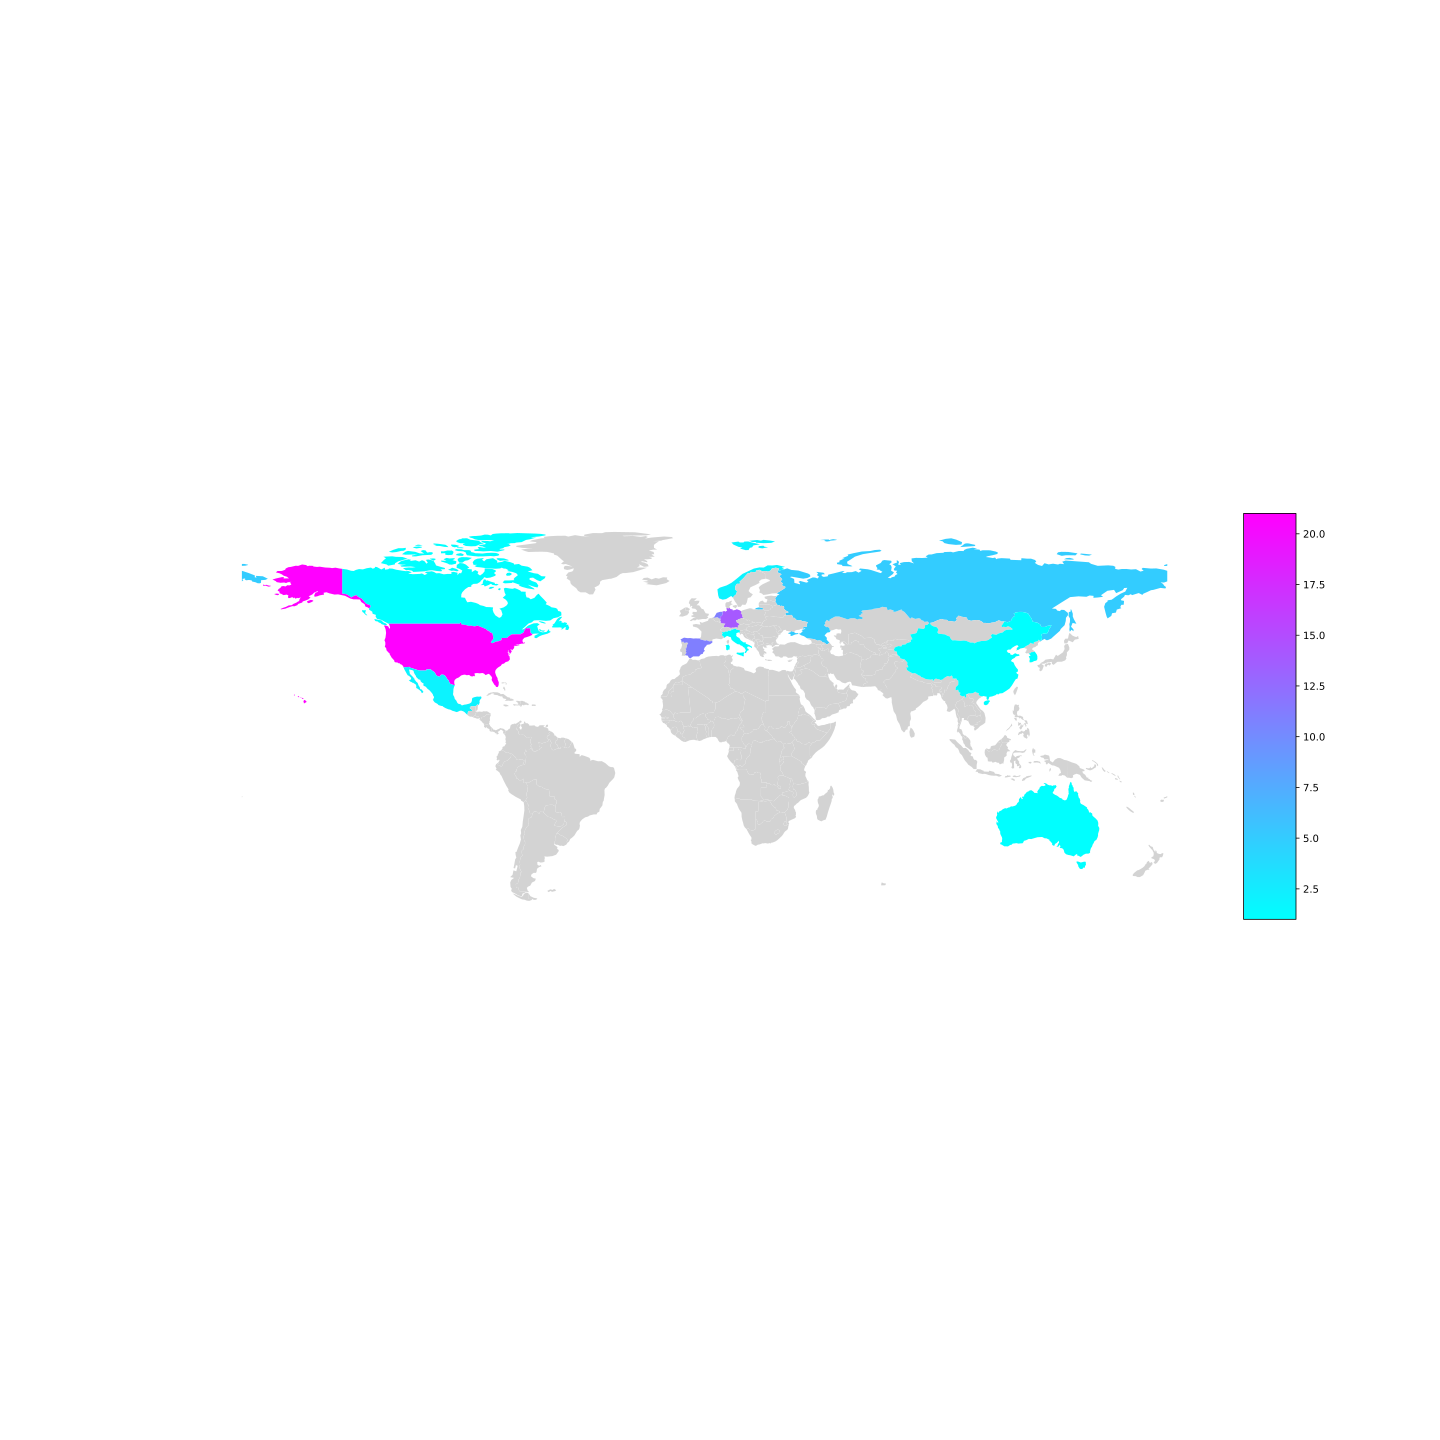
\includegraphics[width=\textwidth]{reports/figures/surveys_per_country.png}
     \caption{Graphic of the number of survey per country}
    \label{fig: surveys_per_country}
\end{figure}


As we could see in this section in the analysis of the meta data of the articles in the review, there are few issues that one has to mind when interpreting the results in the upcoming section. We saw an increasing trend in research, that will most likely not stop in the next years, as the important of mobile internet is still increasing [citation]. We also saw that there is a lag in the time from survey operation to publicaiton of average three years, that we have to mind when interpreting the results. Other possible biases are induced by the concentration of authors and professional survey operators, that could possibly skew the results. One last important factor we have identified is the misisng representativity of the countries survey were operated in, so that the results of review are limited to a few countries. Therefore we have identified future reserach projects, where one reopreats the experiments in other countries and in newer time to test and eventually update the results. 


In this section we gonna discuss the results of the review and give an overview of fully missing dimensions, that could be concentrated in further reswearch.

One important dimension is the  multi mode setting that will likely be there to stay. More and more people are using it and theregore this is an interesting reserach that is already discussed a lot int his review, comparing the quality and particiapnts of mobile aprtiviapnts compared to pc user.

An important dimension for research and other survey operator that is misisng are survey costs and temporal efforts for survey taking. There already exists comparison between online and other modes []. But it coßuld be interesting to see if smartphones and maybe mobile apps could help in reducing these dimension. Especially the usage of app and progressive web app (push) will be an interesting research area to further exploit the advantages of smartphone device. 






